% ==============================================================================
% Example 08: Joint - Constraint System and Joint Types
% ==============================================================================

\section{Example 08: Joint}

\subsection{Overview and Basic Information}

\begin{table}[h]
\centering
\begin{tabular}{|l|l|}
\hline
\textbf{Aspect} & \textbf{Details} \\
\hline
\textbf{Original} & \texttt{snippets/snippetjoint/SnippetJoint.cpp} \\
\textbf{Ported} & \texttt{examples/example\_joint.cpp} \\
\textbf{Difficulty} & ⭐⭐⭐ (Advanced) \\
\textbf{Module} & Joint - Constraint System \\
\textbf{Features} & 6 joint types, Limits, Motors, Breakable joints \\
\hline
\end{tabular}
\end{table}

\subsection{Functional Description}

\subsubsection{Joint Types in PhysX}

PhysX provides 6 core joint types:

\begin{table}[h]
\centering
\begin{tabular}{|l|l|l|}
\hline
\textbf{Joint Type} & \textbf{DOF} & \textbf{Use Cases} \\
\hline
Spherical & 3 rotation & Pendulums, ragdoll shoulders \\
Fixed & 0 & Welded connections \\
Revolute & 1 rotation & Doors, wheels, hinges \\
Prismatic & 1 translation & Pistons, elevators \\
Distance & 1 (variable) & Springs, ropes \\
D6 & 0-6 configurable & Custom constraints \\
\hline
\end{tabular}
\caption{PhysX Joint Types}
\end{table}

\subsubsection{Physics Concepts}

\paragraph{Constraint Equations}

Joints enforce constraints through the iterative solver:
\begin{equation}
\mathbf{C}(\mathbf{q}) = 0
\end{equation}

Where $\mathbf{C}$ = constraint function, $\mathbf{q}$ = generalized coordinates.

For a spherical joint at world position $\mathbf{p}$:
\begin{equation}
\mathbf{C} = \mathbf{p}_1 - \mathbf{p}_2 = \mathbf{0}
\end{equation}

\paragraph{Revolute Joint Math}

Revolute joint allows rotation around axis $\mathbf{a}$:
\begin{equation}
\text{DOF} = 1, \quad \theta \in [\theta_{min}, \theta_{max}]
\end{equation}

Angular limit cone:
\begin{equation}
|\theta - \theta_0| \leq \Delta\theta_{limit}
\end{equation}

\paragraph{Joint Motors}

Motor applies torque to reach target:
\begin{equation}
\tau = K_p(\theta_{target} - \theta) - K_d \dot{\theta}
\end{equation}

Where $K_p$ = stiffness, $K_d$ = damping.

%------------------------------------------------------------------------------

\subsection{Code Comparison}

\textbf{Original PhysX:}
\begin{lstlisting}[caption={Direct joint creation}]
// Create revolute joint manually
PxRevoluteJoint* joint = PxRevoluteJointCreate(
    *gPhysics,
    actor0, PxTransform(PxVec3(0, 0, 0)),
    actor1, PxTransform(PxVec3(0, 0, 0))
);

// Set angle limit
joint->setRevoluteJointFlag(
    PxRevoluteJointFlag::eLIMIT_ENABLED, true);
PxJointAngularLimitPair limit(-PxPi/4, PxPi/4, 0.01f);
joint->setLimit(limit);

// Set motor
joint->setRevoluteJointFlag(
    PxRevoluteJointFlag::eDRIVE_ENABLED, true);
joint->setDriveVelocity(2.0f);
joint->setDriveForceLimit(100.0f);
\end{lstlisting}

\textbf{Wrapper:}
\begin{lstlisting}[caption={Config-driven joint creation}]
JointManager jointMgr;

// Configure revolute joint
RevoluteJointConfig config;
config.enableLimit = true;
config.lowerAngle = -PxPi/4;
config.upperAngle = PxPi/4;
config.limitStiffness = 100.0f;
config.enableMotor = true;
config.motorVelocity = 2.0f;
config.motorForceLimit = 100.0f;

// Create joint
PxRevoluteJoint* joint = jointMgr.createRevoluteJoint(
    actor0, PxTransform(PxVec3(0, 0, 0)),
    actor1, PxTransform(PxVec3(0, 0, 0)),
    config
);
\end{lstlisting}

%------------------------------------------------------------------------------

\subsection{Core Class Analysis}

\subsubsection{Joint Configuration Structures}

\begin{lstlisting}[caption={Spherical joint config}]
struct SphericalJointConfig {
    bool enableLimit = false;
    PxReal yAngleLimit = PxPi / 4.0f;  // Cone Y
    PxReal zAngleLimit = PxPi / 4.0f;  // Cone Z
    PxReal limitStiffness = 100.0f;
    PxReal limitDamping = 10.0f;
    PxReal contactDistance = 0.05f;
};
\end{lstlisting}

\begin{lstlisting}[caption={Revolute joint config}]
struct RevoluteJointConfig {
    bool enableLimit = false;
    PxReal lowerAngle = -PxPi / 2.0f;
    PxReal upperAngle = PxPi / 2.0f;
    PxReal limitStiffness = 100.0f;
    PxReal limitDamping = 10.0f;

    bool enableMotor = false;
    PxReal motorVelocity = 0.0f;
    PxReal motorForceLimit = PX_MAX_F32;
    bool motorFreeSpin = false;
};
\end{lstlisting}

\begin{lstlisting}[caption={D6 joint config}]
struct D6JointConfig {
    // Motion axes
    PxD6Motion::Enum motionX = PxD6Motion::eLOCKED;
    PxD6Motion::Enum motionY = PxD6Motion::eLOCKED;
    PxD6Motion::Enum motionZ = PxD6Motion::eLOCKED;
    PxD6Motion::Enum motionTwist = PxD6Motion::eLOCKED;
    PxD6Motion::Enum motionSwing1 = PxD6Motion::eLOCKED;
    PxD6Motion::Enum motionSwing2 = PxD6Motion::eLOCKED;

    // Linear limits
    PxReal linearLimitValue = 1.0f;
    PxReal linearLimitStiffness = 100.0f;

    // Angular limits
    PxReal twistLowerAngle = -PxPi / 4.0f;
    PxReal twistUpperAngle = PxPi / 4.0f;
    PxReal swingYAngle = PxPi / 4.0f;
    PxReal swingZAngle = PxPi / 4.0f;
};
\end{lstlisting}

\subsubsection{JointManager Core Methods}

\begin{lstlisting}[caption={JointManager API}]
class JointManager {
public:
    // Spherical joint (ball-and-socket)
    PxSphericalJoint* createSphericalJoint(
        PxRigidActor* actor0, const PxTransform& localFrame0,
        PxRigidActor* actor1, const PxTransform& localFrame1,
        const SphericalJointConfig& config
    );

    // Fixed joint (welded)
    PxFixedJoint* createFixedJoint(
        PxRigidActor* actor0, const PxTransform& localFrame0,
        PxRigidActor* actor1, const PxTransform& localFrame1,
        const FixedJointConfig& config
    );

    // Revolute joint (hinge)
    PxRevoluteJoint* createRevoluteJoint(
        PxRigidActor* actor0, const PxTransform& localFrame0,
        PxRigidActor* actor1, const PxTransform& localFrame1,
        const RevoluteJointConfig& config
    );

    // Prismatic joint (slider)
    PxPrismaticJoint* createPrismaticJoint(
        PxRigidActor* actor0, const PxTransform& localFrame0,
        PxRigidActor* actor1, const PxTransform& localFrame1,
        const PrismaticJointConfig& config
    );

    // Distance joint (spring/rope)
    PxDistanceJoint* createDistanceJoint(
        PxRigidActor* actor0, const PxTransform& localFrame0,
        PxRigidActor* actor1, const PxTransform& localFrame1,
        const DistanceJointConfig& config
    );

    // D6 joint (six DOF)
    PxD6Joint* createD6Joint(
        PxRigidActor* actor0, const PxTransform& localFrame0,
        PxRigidActor* actor1, const PxTransform& localFrame1,
        const D6JointConfig& config
    );

    // Breakable joint wrapper
    void setBreakForce(PxJoint* joint, PxReal force, PxReal torque);
    bool isJointBroken(const PxJoint* joint) const;

    // Chain creation
    std::vector<PxJoint*> createJointChain(
        PxRigidActor* start,
        const std::vector<PxRigidActor*>& actors,
        JointType type,
        const void* config
    );
};
\end{lstlisting}

%------------------------------------------------------------------------------

\subsection{Visual Diagrams}

\begin{figure}[h]
\centering
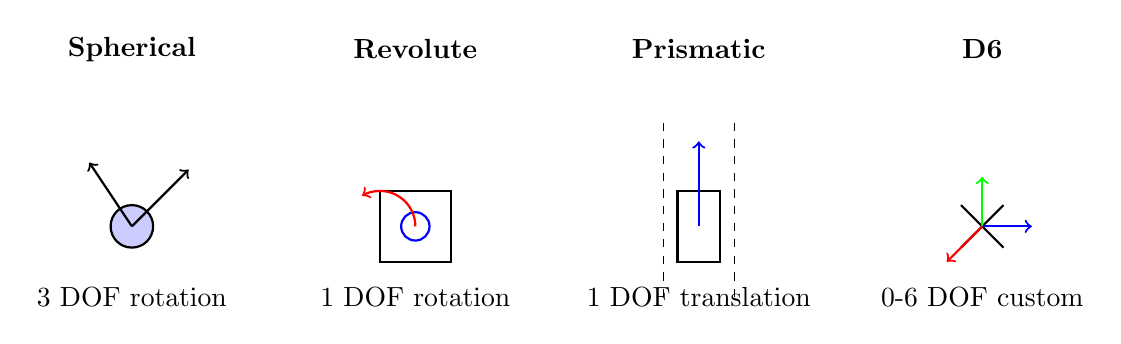
\begin{tikzpicture}[scale=0.9]
    % Spherical
    \begin{scope}[xshift=-6cm]
        \node at (0, 2.5) {\textbf{Spherical}};
        \fill[blue!20] (0, 0) circle (0.3);
        \draw[thick] (0, 0) circle (0.3);
        \draw[->, thick] (0, 0) -- (0.8, 0.8);
        \draw[->, thick] (0, 0) -- (-0.6, 0.9);
        \node at (0, -1) {3 DOF rotation};
    \end{scope}

    % Revolute
    \begin{scope}[xshift=-2cm]
        \node at (0, 2.5) {\textbf{Revolute}};
        \draw[thick] (-0.5, -0.5) rectangle (0.5, 0.5);
        \draw[thick, blue] (0, 0) circle (0.2);
        \draw[->, thick, red] (0, 0) arc (0:120:0.5);
        \node at (0, -1) {1 DOF rotation};
    \end{scope}

    % Prismatic
    \begin{scope}[xshift=2cm]
        \node at (0, 2.5) {\textbf{Prismatic}};
        \draw[thick] (-0.3, -0.5) rectangle (0.3, 0.5);
        \draw[->, thick, blue] (0, 0) -- (0, 1.2);
        \draw[dashed] (-0.5, -1) -- (-0.5, 1.5);
        \draw[dashed] (0.5, -1) -- (0.5, 1.5);
        \node at (0, -1) {1 DOF translation};
    \end{scope}

    % D6
    \begin{scope}[xshift=6cm]
        \node at (0, 2.5) {\textbf{D6}};
        \draw[thick] (-0.3, -0.3) -- (0.3, 0.3);
        \draw[thick] (0.3, -0.3) -- (-0.3, 0.3);
        \draw[->, thick, blue] (0, 0) -- (0.7, 0);
        \draw[->, thick, green] (0, 0) -- (0, 0.7);
        \draw[->, thick, red] (0, 0) -- (-0.5, -0.5);
        \node at (0, -1) {0-6 DOF custom};
    \end{scope}
\end{tikzpicture}
\caption{Joint Types Visualization}
\end{figure}

%------------------------------------------------------------------------------

\subsection{Usage Methodology}

\subsubsection{Creating a Door (Revolute Joint)}

\begin{lstlisting}[caption={Door with revolute joint}]
JointManager jointMgr;

// Door frame (static)
PxRigidStatic* frame = physics.createRigidStatic(
    PxTransform(PxVec3(0, 2, 0)));

// Door (dynamic)
PxRigidDynamic* door = createBox(physics, scene,
    PxVec3(1, 2, 0), PxVec3(1, 2, 0.1f), 50.0f, material);

// Revolute joint with 90° limit
RevoluteJointConfig config;
config.enableLimit = true;
config.lowerAngle = 0;
config.upperAngle = PxPi / 2.0f;  // 90 degrees

PxRevoluteJoint* hinge = jointMgr.createRevoluteJoint(
    frame, PxTransform(PxVec3(0, 0, 0)),
    door, PxTransform(PxVec3(-1, 0, 0)),  // Hinge at left edge
    config
);
\end{lstlisting}

\subsubsection{Creating a Rope Chain}

\begin{lstlisting}[caption={Rope using distance joints}]
JointManager jointMgr;

std::vector<PxRigidDynamic*> links;
PxVec3 startPos(0, 20, 0);

// Create rope links
for (int i = 0; i < 10; i++) {
    PxRigidDynamic* link = createSphere(physics, scene,
        startPos + PxVec3(0, -i * 0.5f, 0),
        0.2f, 10.0f, material);
    links.push_back(link);
}

// Connect with distance joints
for (size_t i = 0; i < links.size() - 1; i++) {
    DistanceJointConfig config;
    config.minDistance = 0.4f;
    config.maxDistance = 0.6f;
    config.stiffness = 100.0f;
    config.damping = 10.0f;

    jointMgr.createDistanceJoint(
        links[i], PxTransform(PxVec3(0, -0.25f, 0)),
        links[i+1], PxTransform(PxVec3(0, 0.25f, 0)),
        config
    );
}
\end{lstlisting}

%------------------------------------------------------------------------------

\subsection{Performance Considerations}

\begin{table}[h]
\centering
\begin{tabular}{|l|c|l|}
\hline
\textbf{Optimization} & \textbf{Impact} & \textbf{Technique} \\
\hline
Solver iterations & High & Lower for non-critical joints \\
Break force & Medium & Use breakable joints sparingly \\
Projection & High & Enable for long chains \\
Joint count & High & Merge fixed joints when possible \\
\hline
\end{tabular}
\caption{Joint Performance Tips}
\end{table}

%------------------------------------------------------------------------------

\subsection{Feature Completeness}

\begin{table}[h]
\centering
\begin{tabular}{|l|c|c|}
\hline
\textbf{Feature} & \textbf{Original} & \textbf{Wrapper} \\
\hline
All 6 joint types & ✓ & ✓ \\
Angle/distance limits & ✓ & ✓ \\
Motors/drives & ✓ & ✓ \\
Breakable joints & ✓ & ✓ \\
Config-driven API & ✗ & ✓ \\
Joint chains & ✗ & ✓ \\
Unified manager & ✗ & ✓ \\
\hline
\end{tabular}
\end{table}

%------------------------------------------------------------------------------

\subsection{Quality Assessment}

\begin{table}[h]
\centering
\begin{tabular}{|l|c|}
\hline
\textbf{Category} & \textbf{Rating} \\
\hline
Functional Fidelity & ⭐⭐⭐⭐⭐ \\
Code Quality & ⭐⭐⭐⭐⭐ \\
Usability & ⭐⭐⭐⭐⭐ \\
Documentation & ⭐⭐⭐⭐⭐ \\
\hline
\end{tabular}
\end{table}

\textbf{Approval Status:} \textcolor{green}{\textbf{APPROVED}} ✓

%==============================================================================
% End of Example 08: Joint
%==============================================================================
